\section{Interfaces de anotación y operación}
\label{app:interfaces}

La Fig.~\ref{fig:interfaz_etiquetado} muestra la versión final del entorno de revisión humana con un chunk real del corpus. La propuesta de DeepSeek Pro aparece antes de decidir y deja tres acciones explícitas: aceptarla, rechazar el caso o modificar las categorías y señales antes de guardar la versión humana. El contador corresponde a la campaña integrada que alimenta esta interfaz.

\begin{figure}[H]
\centering
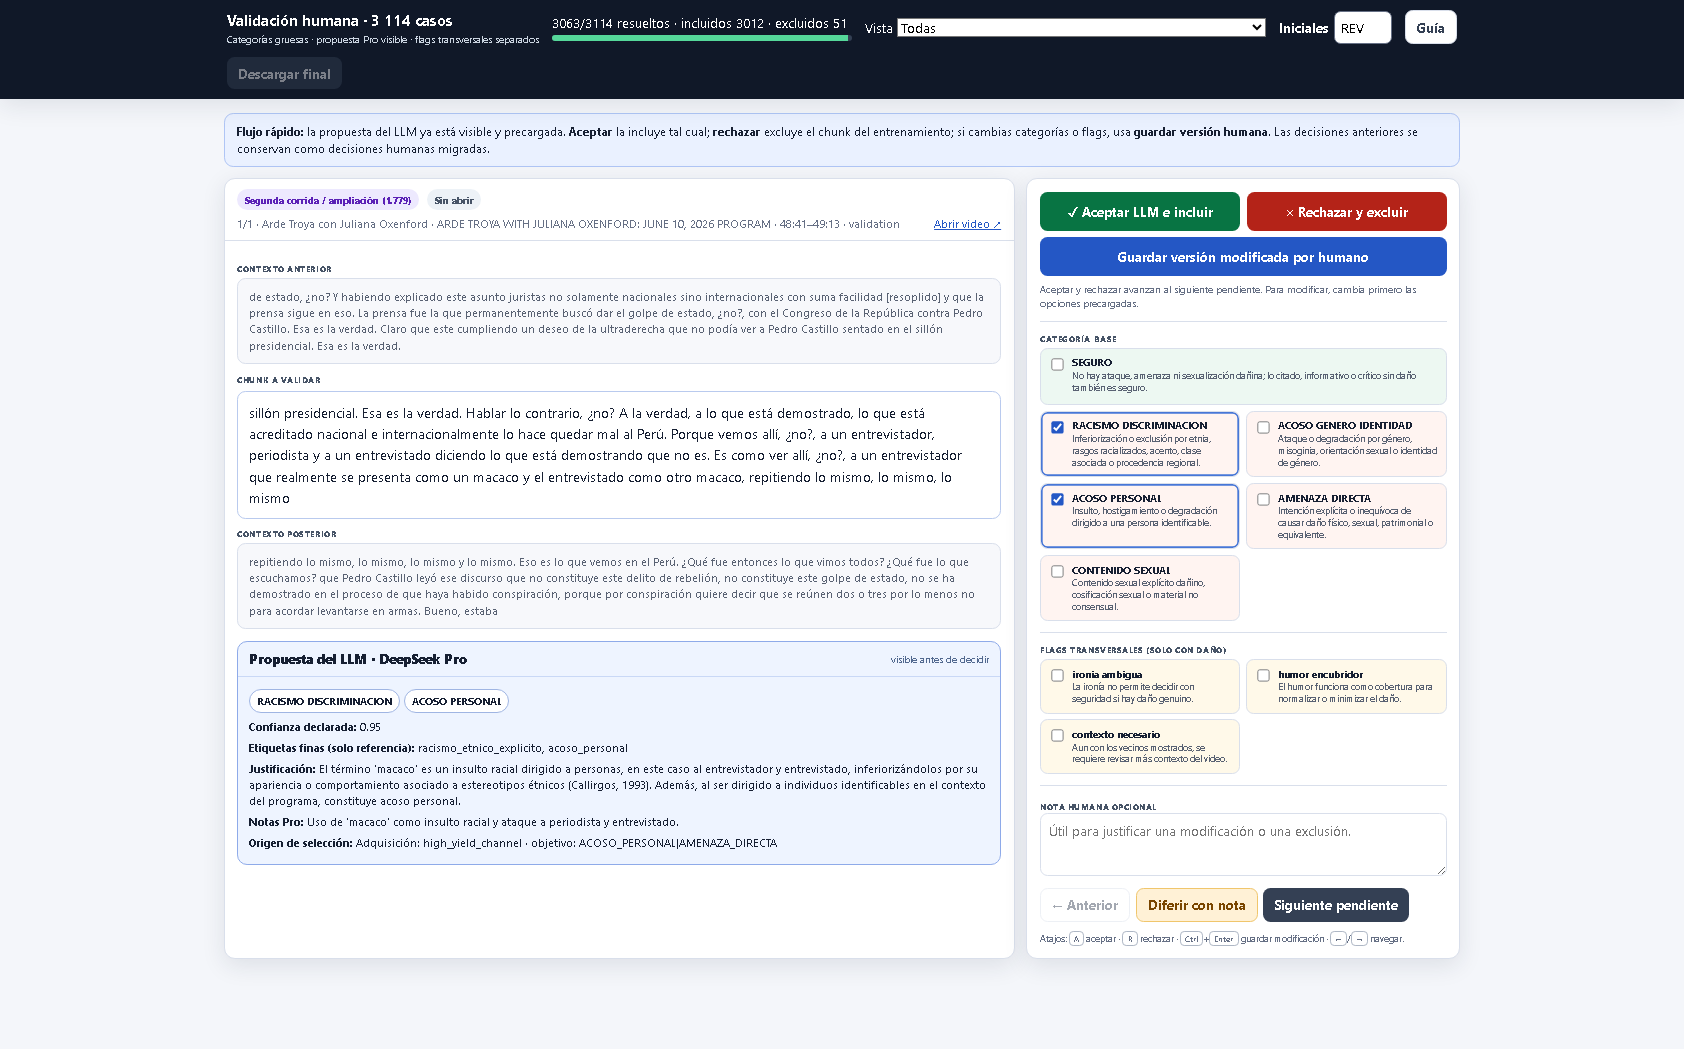
\includegraphics[width=.98\linewidth,height=.78\textheight,keepaspectratio]{figuras/captura_entorno_etiquetado.png}
\caption{Entorno final de revisión humana: texto y contexto, propuesta visible del LLM y controles para aceptar, rechazar o modificar. Captura local del artefacto del proyecto con un registro real.}
\label{fig:interfaz_etiquetado}
\end{figure}

\clearpage

La Fig.~\ref{fig:interfaz_operacion} presenta el demostrador después de enviar por su formulario un chunk real de validación al servidor del paquete desplegable. Qwen3--LoRA asigna 0,94 a contenido sexual; la política operativa conserva el caso como alerta de confianza baja y solicita revisión por su cercanía al umbral. La pantalla muestra la entrada enviada, la respuesta del servidor, los puntajes por categoría y los controles humanos. Cuando la entrada es un video de YouTube, la misma interfaz añade el reproductor y los enlaces temporales a los fragmentos señalados.

\begin{figure}[H]
\centering
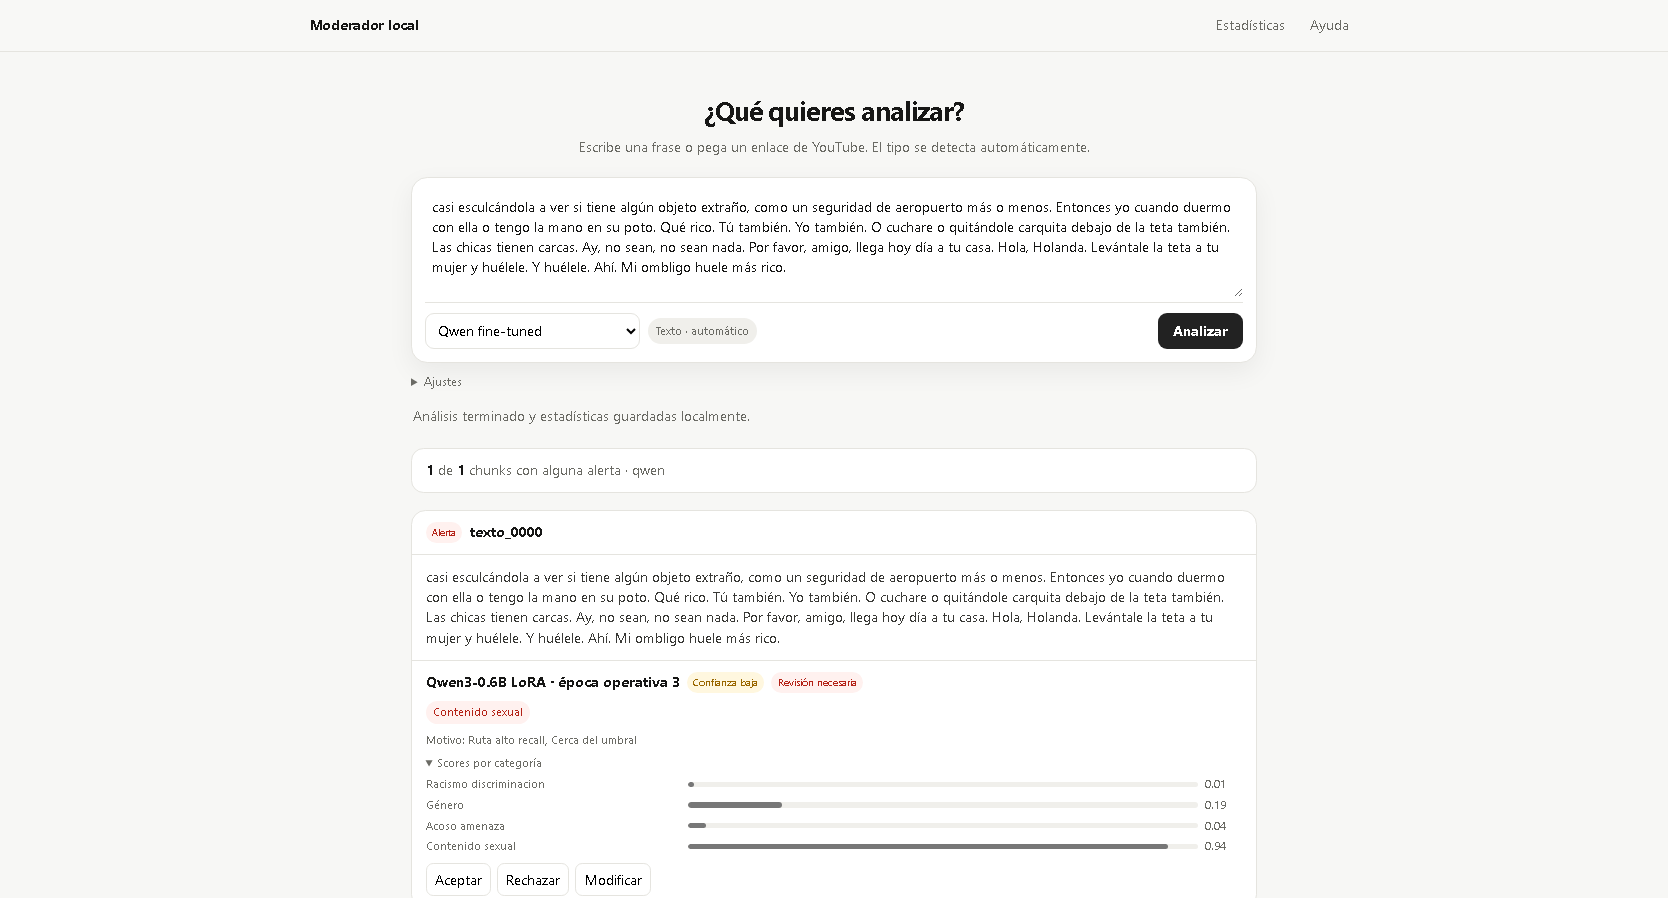
\includegraphics[width=.98\linewidth,height=.78\textheight,keepaspectratio]{figuras/captura_entorno_operacion.png}
\caption{Ejecución real del servidor del paquete desplegable: el formulario envía un chunk de validación, registra una inferencia nueva y muestra la alerta, los puntajes de Qwen3--LoRA y las acciones de revisión humana.}
\label{fig:interfaz_operacion}
\end{figure}
